\documentclass{article} 
\usepackage{graphicx}

\begin{document}
\title{My First LaTeX Document}
\author{Dr. Milaan Parmar}

\maketitle
\begin{abstract}
Smartphones are increasingly being used to store personal information as well as to access sensitive data from the Internet and the cloud. Establishment of the identity of a user requesting information from smartphones is a prerequisite for  secure systems in such scenarios. In the past, keystroke-based user identifiation has been successfully deployed on production-level mobile devices to mitigate the risks associated with naive username/password based authentication. However, these approaches have two major limitations: they are not applicable to services where authentication occurs outside the domain of the mobile
device such as web-based services; and they often overly tax the limited computational capabilities of mobile devices.

In this paper, we propose a protocol for keystroke dynamics analysis which allows web-based applications to make use of remote attestation and delegated keystroke analysis. The end result is an efficient keystroke-based user identification mechanism that strengthens traditional password protected services
while mitigating the risks of user profiling by collaborating malicious web
services. We present a prototype implementation of our protocol using
the popular Android operating system for smartphones.
\end{abstract}

\section{Introduction} 
This is going to be a normal paragraph in our introduction. 

\subsection{Some Background} 
Some more stuff. 

\subsubsection{Drilled Down}\label{sec:drilled-down}
More information here. 

\section{Background}\label{sec:background}

\subsection{More Stuff: Tables and Figures}
To insert a figure, you can use the TeXnicecenter menus. 

\begin{figure}
	\centering
		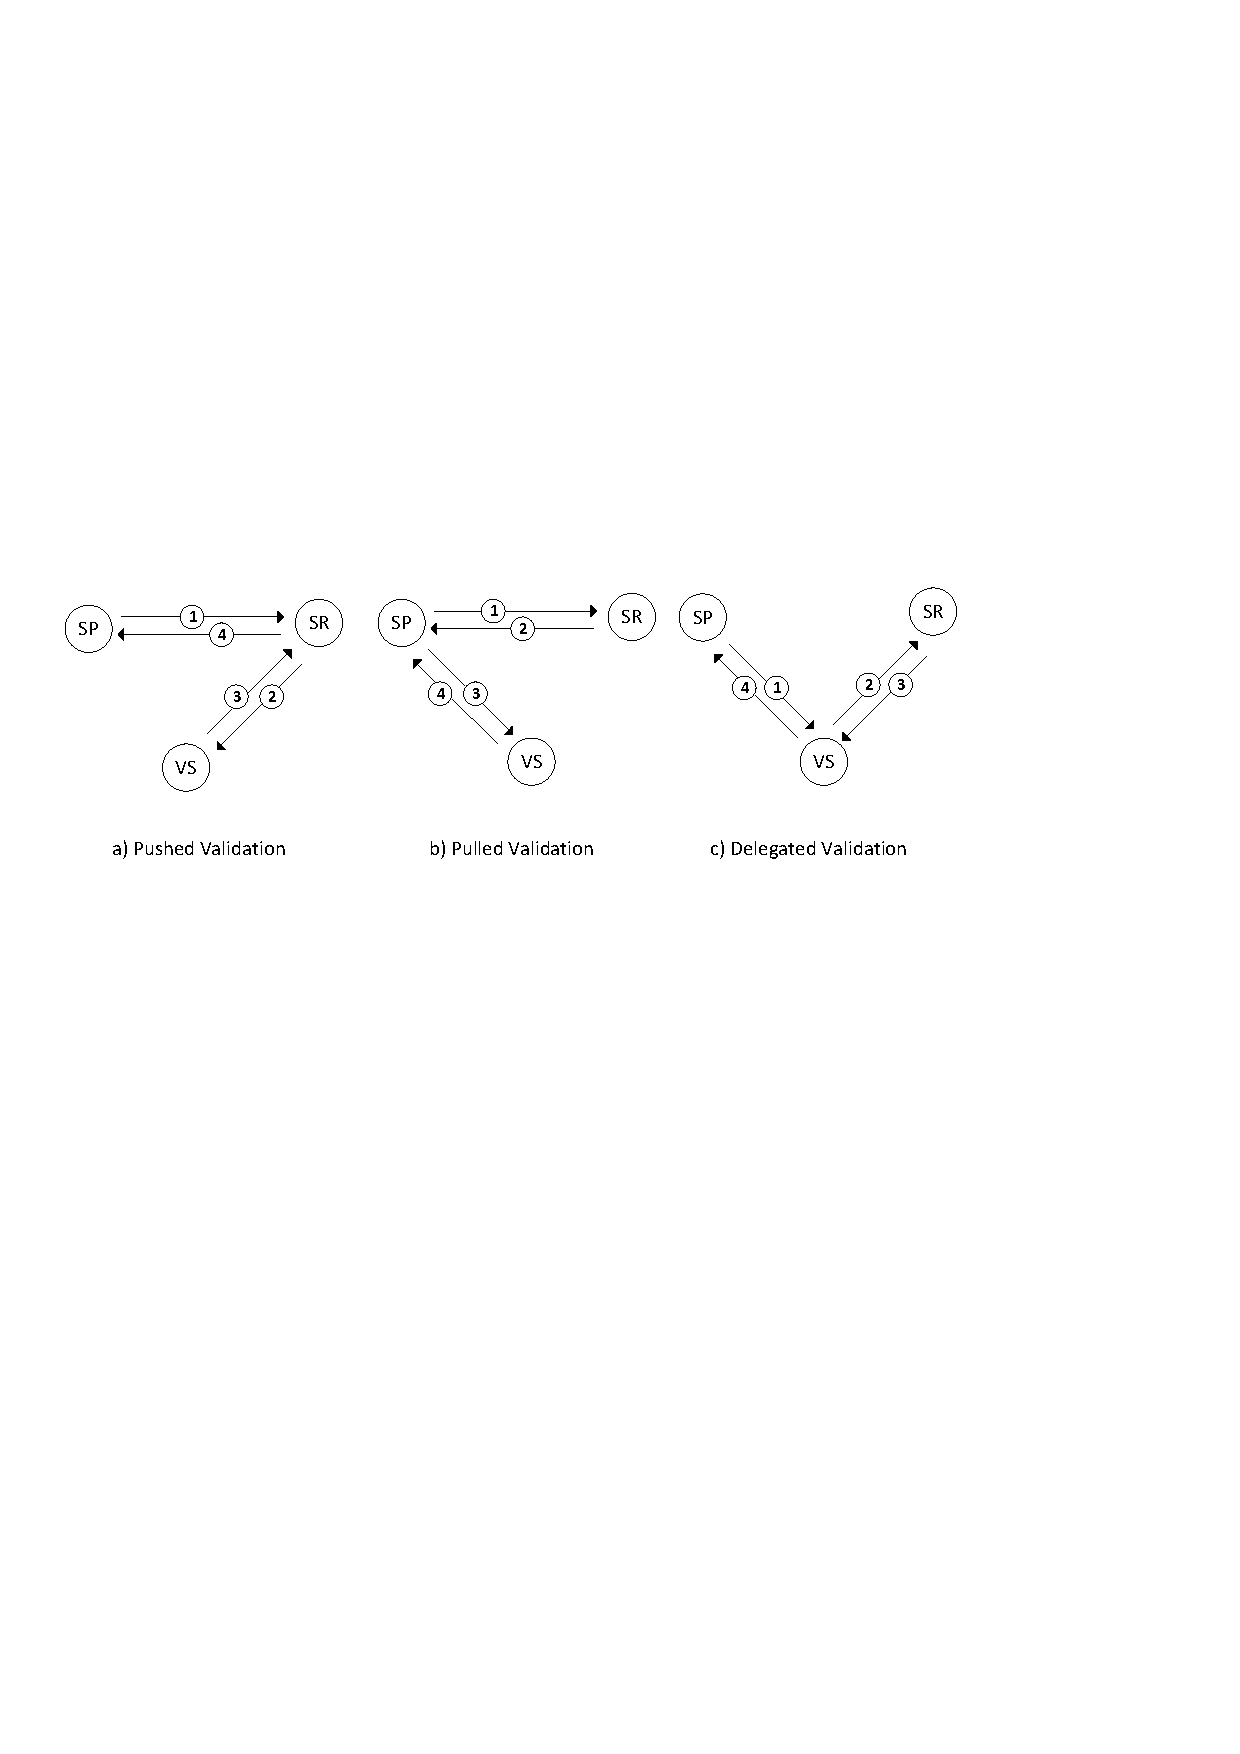
\includegraphics[width=1.00\textwidth]{att-models-base.pdf}
	\caption{My First Figure}
	\label{fig:att-models-base}
\end{figure}

Now for a table! 

\begin{table}
	\centering
		\begin{tabular}{|l|c|c|c|}
		\hline 
		Head 1 & Head 2 & Head 3 & Head 4   \\\hline 
		1      &      2 & 3      & 4 \\			
		\hline
		\end{tabular}
	\caption{My First Table}
	\label{tab:MyFirstTable}
\end{table}

\subsection{More Stuff} 
Some text here that wants to refer to Table~\ref{tab:MyFirstTable}. You can also refer to the Figure~\ref{fig:att-models-base}. When you want to refer to a previous section, you can use the \verb|\ref| command again. Section~\ref{sec:background} and Section~\ref{sec:drilled-down}. 

\subsection{Sub section through input command}
This comes from a separate file. Notice that I have this subsection included in the Navigator.  

\end{document} 